%<dscrpt>Fichier de déclarations Latex à inclure au début d'un élément de cours.</dscrpt>

\documentclass[a4paper]{article}
\usepackage[hmargin={1.8cm,1.8cm},vmargin={2.4cm,2.4cm},headheight=13.1pt]{geometry}

%includeheadfoot,scale=1.1,centering,hoffset=-0.5cm,
\usepackage[pdftex]{graphicx,color}
\usepackage[french]{babel}
%\selectlanguage{french}
\addto\captionsfrench{
  \def\contentsname{Plan}
}
\usepackage{fancyhdr}
\usepackage{floatflt}
\usepackage{amsmath}
\usepackage{amssymb}
\usepackage{amsthm}
\usepackage{stmaryrd}
%\usepackage{ucs}
\usepackage[utf8]{inputenc}
%\usepackage[latin1]{inputenc}
\usepackage[T1]{fontenc}


\usepackage{titletoc}
%\contentsmargin{2.55em}
\dottedcontents{section}[2.5em]{}{1.8em}{1pc}
\dottedcontents{subsection}[3.5em]{}{1.2em}{1pc}
\dottedcontents{subsubsection}[5em]{}{1em}{1pc}

\usepackage[pdftex,colorlinks={true},urlcolor={blue},pdfauthor={remy Nicolai},bookmarks={true}]{hyperref}
\usepackage{makeidx}

\usepackage{multicol}
\usepackage{multirow}
\usepackage{wrapfig}
\usepackage{array}
\usepackage{subfig}


%\usepackage{tikz}
%\usetikzlibrary{calc, shapes, backgrounds}
%pour la présentation du pseudo-code
% !!!!!!!!!!!!!!      le package n'est pas présent sur le serveur sous fedora 16 !!!!!!!!!!!!!!!!!!!!!!!!
%\usepackage[french,ruled,vlined]{algorithm2e}

%pr{\'e}sentation du compteur de niveau 2 dans les listes
\makeatletter
\renewcommand{\labelenumii}{\theenumii.}
\renewcommand{\thesection}{\Roman{section}.}
\renewcommand{\thesubsection}{\arabic{subsection}.}
\renewcommand{\thesubsubsection}{\arabic{subsubsection}.}
\makeatother


%dimension des pages, en-t{\^e}te et bas de page
%\pdfpagewidth=20cm
%\pdfpageheight=14cm
%   \setlength{\oddsidemargin}{-2cm}
%   \setlength{\voffset}{-1.5cm}
%   \setlength{\textheight}{12cm}
%   \setlength{\textwidth}{25.2cm}
   \columnsep=1cm
   \columnseprule=0.5pt

%En tete et pied de page
\pagestyle{fancy}
\lhead{MPSI-\'Eléments de cours}
\rhead{\today}
%\rhead{25/11/05}
\lfoot{\tiny{Cette création est mise à disposition selon le Contrat\\ Paternité-Pas d'utilisations commerciale-Partage des Conditions Initiales à l'Identique 2.0 France\\ disponible en ligne http://creativecommons.org/licenses/by-nc-sa/2.0/fr/
} }
\rfoot{\tiny{Rémy Nicolai \jobname}}


\newcommand{\baseurl}{http://back.maquisdoc.net/data/cours\_nicolair/}
\newcommand{\urlexo}{http://back.maquisdoc.net/data/exos_nicolair/}
\newcommand{\urlcours}{https://maquisdoc-math.fra1.digitaloceanspaces.com/}

\newcommand{\N}{\mathbb{N}}
\newcommand{\Z}{\mathbb{Z}}
\newcommand{\C}{\mathbb{C}}
\newcommand{\R}{\mathbb{R}}
\newcommand{\D}{\mathbb{D}}
\newcommand{\K}{\mathbf{K}}
\newcommand{\Q}{\mathbb{Q}}
\newcommand{\F}{\mathbf{F}}
\newcommand{\U}{\mathbb{U}}
\newcommand{\p}{\mathbb{P}}


\newcommand{\card}{\mathop{\mathrm{Card}}}
\newcommand{\Id}{\mathop{\mathrm{Id}}}
\newcommand{\Ker}{\mathop{\mathrm{Ker}}}
\newcommand{\Vect}{\mathop{\mathrm{Vect}}}
\newcommand{\cotg}{\mathop{\mathrm{cotan}}}
\newcommand{\sh}{\mathop{\mathrm{sh}}}
\newcommand{\ch}{\mathop{\mathrm{ch}}}
\newcommand{\argsh}{\mathop{\mathrm{argsh}}}
\newcommand{\argch}{\mathop{\mathrm{argch}}}
\newcommand{\tr}{\mathop{\mathrm{tr}}}
\newcommand{\rg}{\mathop{\mathrm{rg}}}
\newcommand{\rang}{\mathop{\mathrm{rg}}}
\newcommand{\Mat}{\mathop{\mathrm{Mat}}}
\newcommand{\MatB}[2]{\mathop{\mathrm{Mat}}_{\mathcal{#1}}\left( #2\right) }
\newcommand{\MatBB}[3]{\mathop{\mathrm{Mat}}_{\mathcal{#1} \mathcal{#2}}\left( #3\right) }
\renewcommand{\Re}{\mathop{\mathrm{Re}}}
\renewcommand{\Im}{\mathop{\mathrm{Im}}}
\renewcommand{\th}{\mathop{\mathrm{th}}}
\newcommand{\repere}{$(O,\overrightarrow{i},\overrightarrow{j},\overrightarrow{k})$}
\newcommand{\cov}{\mathop{\mathrm{Cov}}}

\newcommand{\absolue}[1]{\left| #1 \right|}
\newcommand{\fonc}[5]{#1 : \begin{cases}#2 \rightarrow #3 \\ #4 \mapsto #5 \end{cases}}
\newcommand{\depar}[2]{\dfrac{\partial #1}{\partial #2}}
\newcommand{\norme}[1]{\left\| #1 \right\|}
\newcommand{\se}{\geq}
\newcommand{\ie}{\leq}
\newcommand{\trans}{\mathstrut^t\!}
\newcommand{\val}{\mathop{\mathrm{val}}}
\newcommand{\grad}{\mathop{\overrightarrow{\mathrm{grad}}}}

\newtheorem*{thm}{Théorème}
\newtheorem{thmn}{Théorème}
\newtheorem*{prop}{Proposition}
\newtheorem{propn}{Proposition}
\newtheorem*{pa}{Présentation axiomatique}
\newtheorem*{propdef}{Proposition - Définition}
\newtheorem*{lem}{Lemme}
\newtheorem{lemn}{Lemme}

\theoremstyle{definition}
\newtheorem*{defi}{Définition}
\newtheorem*{nota}{Notation}
\newtheorem*{exple}{Exemple}
\newtheorem*{exples}{Exemples}


\newenvironment{demo}{\renewcommand{\proofname}{Preuve}\begin{proof}}{\end{proof}}
%\renewcommand{\proofname}{Preuve} doit etre après le begin{document} pour fonctionner

\theoremstyle{remark}
\newtheorem*{rem}{Remarque}
\newtheorem*{rems}{Remarques}

\renewcommand{\indexspace}{}
\renewenvironment{theindex}
  {\section*{Index} %\addcontentsline{toc}{section}{\protect\numberline{0.}{Index}}
   \begin{multicols}{2}
    \begin{itemize}}
  {\end{itemize} \end{multicols}}


%pour annuler les commandes beamer
\renewenvironment{frame}{}{}
\newcommand{\frametitle}[1]{}
\newcommand{\framesubtitle}[1]{}

\newcommand{\debutcours}[2]{
  \chead{#1}
  \begin{center}
     \begin{huge}\textbf{#1}\end{huge}
     \begin{Large}\begin{center}Rédaction incomplète. Version #2\end{center}\end{Large}
  \end{center}
  %\section*{Plan et Index}
  %\begin{frame}  commande beamer
  \tableofcontents
  %\end{frame}   commande beamer
  \printindex
}


\makeindex
\begin{document}
\noindent

\debutcours{Sous-espaces affines d'un espace vectoriel}{0.2 \tiny{\today}}

Ce texte est la dernière partie du cours d'algèbre linéaire. La partie précédente est \href{\baseurl C9587.pdf}{Applications linéaires et dimension finie}.

\section{Espace vectoriel comme ensemble de points}
Les espaces vectoriels fournissent de bons modèles pour pratiquer la géométrie élémentaire \footnote{Des compléments sortis du programme de la mpsi sont présentés dans les documents \href{\baseurl C5727.pdf}{Espaces affines} et \href{\baseurl C2005.pdf}{Géométrie élémentaire du plan}}.\newline
On convient d'appeler \emph{point} un élément d'un $\K$-espace vectoriel (en général $\K = \R$). Les éléments d'un espace vectoriel possèdent donc deux \og casquettes\fg: ils sont à la fois points et vecteurs. On peut adopter des conventions typographiques; par exemple noter les éléments considérés comme des points avec des capitales $A$, $B$, $P\cdots$ et les éléments considérés comme des vecteurs avec des minuscules $u$, $v$, $w\cdots$.\newline
L'utilisation d'une flèche au dessus $\overrightarrow{\phantom{AB}}$ est associée à la soustraction dans l'espace vectoriel. On note
\begin{displaymath}
  \forall (A,B)\in E^2 \text{ (vus comme des points) }, \hspace{0.5cm}
  \overrightarrow{AB} = B - A \text{ (vu comme un vecteur soustraction de deux vecteurs) }
\end{displaymath}
Avec une telle notation, les relations de Chasles \index{relation de Chasles} sont immédiates
\begin{displaymath}
  \forall (A,B,C)\in E^3, \hspace{0.5cm} \overrightarrow{BA} = A - B = -(B-A) = -\overrightarrow{AB},\hspace{0.5cm}
\overrightarrow{AB} + \overrightarrow{BC} = (B-A) + (C-B) = C - A = \overrightarrow{AC}
  \end{displaymath}
On peut noter le rôle particulier joué par le vecteur nul
\begin{displaymath}
  \forall A \in E, \; A = \overrightarrow{0_E A}
\end{displaymath}
\begin{defi}[translation]\index{translation}
  Soit $E$ un $\K$-espace vectoriel et $u\in E$. La translation de vecteur $u$ est l'application
  \begin{displaymath}
    t_u:
    \left\lbrace 
    \begin{aligned}
      E &\rightarrow E \\ M &\mapsto M + u
    \end{aligned}
\right. 
  \end{displaymath}
\end{defi}
\begin{rems}
  \begin{itemize}
    \item Pour tous $A$, $B$, $u$ dans $E$, 
\begin{displaymath}
  \overrightarrow{AB} = u \Leftrightarrow B = A + u \Leftrightarrow B = t_u(A)
\end{displaymath}
    \item Pour tous $u$ et $v$ dans $E$, $t_u \circ t_v = t_{u+v}$.
  \end{itemize}
\end{rems}


\section{Définition d'un sous-espace affine}
\begin{defi}
 Soit $E$ un $\K$-espace vectoriel et $\mathcal A$ une partie de $E$. Pour tout élément $a_0$ de $\mathcal A$, on pose
\begin{displaymath}
 D_{a_0}(\mathcal{A}) = \left\lbrace a- a_0, a\in \mathcal A\right\rbrace = \left\lbrace \overrightarrow{a_0\, a}, a\in \mathcal A\right\rbrace  .
\end{displaymath}
\end{defi}
\begin{rem}
 $D_{a_0}(\mathcal{A})$ est l'ensemble des vecteurs issus de $a_0$ et d'extrémité dans $\mathcal{A}$.
\end{rem}

\begin{defi}
 Soit $E$ un $\K$-espace vectoriel et $A$ une partie de $E$. Pour tout élément $x$ de $E$, on pose
\begin{displaymath}
 x+A = \left\lbrace x+u, u\in A\right\rbrace .
\end{displaymath}
\end{defi}
\begin{rem}
 On regarde $D_{a_0}(\mathcal{A})$ comme un ensemble de vecteurs et $x + A$ comme un ensemble de points. Par définition, pour une partie $\mathcal{A}$ donnée (vue comme un ensemble de points),
\begin{displaymath}
\forall a_0\in \mathcal{A}, \hspace{0.5cm} \mathcal A = a_0 + D_{a_0}(\mathcal{A})=\left\lbrace  a_0 + x, x\in D_{a_0}(\mathcal{A})\right\rbrace 
\end{displaymath}
\end{rem}

\begin{prop}
 Soit $\mathcal A$ une partie d'un $\K$-espace vectoriel $E$. S'il existe un $a_0\in\mathcal A$ tel que $D_{a_0}(\mathcal{A})$ est un sous-espace vectoriel de $E$, alors
\[
 \forall a_1 \in \mathcal A, \; D_{a_1}(\mathcal{A}) = D_{a_0}(\mathcal{A}).
\]
\end{prop}
\begin{demo}
 On doit prouver deux inclusions.
\begin{itemize}
 \item Montrons que $D_{a_1}(\mathcal{A})\subset D_{a_0}(\mathcal{A})$. Soit $u_1\in D_{a_1}(\mathcal{A})$, il existe $\alpha\in \mathcal{A}$ tel que $u_1=\alpha - a_1$. Alors
\begin{displaymath}
 u_1 = \underset{\in D_{a_0}(\mathcal{A})}{\underbrace{\alpha - a_0}} -\underset{\in D_{a_0}(\mathcal{A})}{\underbrace{(a_1-a_0)}} \in D_{a_0}(\mathcal{A}) \hspace{1cm}\text{(stable par addition)}
\end{displaymath}
 \item Montrons que $D_{a_0}(\mathcal{A})\subset D_{a_1}(\mathcal{A})$. Attention, on ne peut pas raisonner comme pour la première inclusion car c'est $D_{a_0}(\mathcal{A})$ qui est un sous-espace vectoriel et non $D_{a_1}(\mathcal{A})$.\newline
Soit $u_0\in D_{a_0}(\mathcal{A})$, il existe $\alpha\in \mathcal{A}$ tel que $u_0=\alpha - a_0$. On peut écrire $u_0$ comme
\begin{displaymath}
 u_0 = (\alpha -a_0 + a_1) -a_1 
\end{displaymath}
On doit montrer que $\alpha -a_0 + a_1 \in \mathcal{A}$. Or:
\begin{displaymath}
\alpha -a_0 + a_1 = \underset{\in D_{a_0}(\mathcal{A})}{\underbrace{\alpha - a_0}} + \underset{\in D_{a_0}(\mathcal{A})}{\underbrace{a_1 - a_0}} + a_0 \in a_0 + D_{a_0}(\mathcal{A}) = \mathcal{A}
\end{displaymath}
car $D_{a_0}(\mathcal{A})$ est stable par addition.
\end{itemize}
\end{demo}
\begin{defi}
 On dira qu'une partie $\mathcal A$ d'un $\K$ espace vectoriel $E$ est un sous-espace affine \index{sous-espace affine} si et seulement si il existe un $a_0\in\mathcal A$ tel que 
\begin{displaymath}
 D_{a_0}(\mathcal{A}) = \left\lbrace a-a_0, a\in \mathcal A\right\rbrace 
\end{displaymath}
est un sous-espace vectoriel de $E$. Ce sous-espace vectoriel, indépendant du $a_0$ d'après la première proposition est appelé la \emph{direction du sous-espace affine}\index{direction d'un sous-espace affine}.
\end{defi}
\begin{rem}
 Un singleton est un sous-espace affine de direction $\{0_E\}$.
\end{rem}
\begin{exple}
 Soit $f\in\mathcal{L}(E,F)$ et $y\in\F$. L'ensemble des solutions dans $E$ d'une équation $f(x) = y$ est vide si $y$ n'est pas dans l'image de $f$ et c'est un sous-espace affine de direction $\ker f$ lorsque $y \in \Im f$. 
\end{exple}
Cet exemple recouvre les cas des équations différentielles linéaires avec second membre, des systèmes linéaires et des polynômes interpolateurs.

\section{Intersection de sous-espaces affines.}
\begin{defi}
 On dira que deux sous-espaces affines sont parallèles lorsque la direction de l'un est incluse dans la direction de l'autre. 
\end{defi}

\begin{propn}\label{sing}
 Soit $\mathcal A$ un sous-espace affine de direction $A$ et $\mathcal B$ un sous-espace affine de direction $B$. Si $\mathcal A\cap \mathcal B$ est non vide, alors $\mathcal A\cap \mathcal B$ est un sous-espace affine de direction $A\cap B$.
\end{propn}
\begin{demo}
Soit $m_0\in \mathcal{A} \cap \mathcal{B}$.
\begin{displaymath}
\forall m \in E,\; m\in \mathcal{A}\cap \mathcal{B}
\Leftrightarrow
\left\lbrace 
\begin{aligned}
  m-m_0 \in& A \\ m-m_0\in& B
\end{aligned}
\right. \Leftrightarrow m-m_0 \in A\cap B .
\end{displaymath}
On en déduit que
\begin{displaymath}
  \left\lbrace m-m_0, \text{ tq } m\in \mathcal{A}\cap \mathcal{B}\right\rbrace = A\cap B .
\end{displaymath}
\end{demo}
\begin{rem}
 Lorsque $A\cap B=\{0_E\}$, l'intersection $\mathcal A \cap \mathcal B$ est soit vide soit réduite à un singleton.
\end{rem}

\begin{propn}\label{somm}
 Soit $\mathcal A$ un sous-espace affine de direction $A$ et $\mathcal B$ un sous-espace affine de direction $B$. Lorsque $A+B=E$, l'intersection $\mathcal A\cap \mathcal B$ est non vide.
\end{propn}
\begin{demo}
Soit $a\in \mathcal{A}$ et $b\in\mathcal{B}$. Comme $A+B=E$, on peut décomposer la différence: 
\[
\exists \alpha\in A \text{ et }\beta\in B \text{ tels que }  b - a = \alpha + \beta \Rightarrow 
 \underset{\in \mathcal{A}}{\underbrace{a + \alpha}} = \underset{\in \mathcal{B}}{\underbrace{b + (-\beta)}} \in \mathcal{A} \cap \mathcal{B}.
\]
\end{demo}

\begin{propn}\label{supp}
 Soit $\mathcal A$ un sous-espace affine de direction $A$ et $\mathcal B$ un sous-espace affine de direction $B$. Lorsque $A$ et $B$ sont supplémentaires, l'intersection $\mathcal A\cap \mathcal B$ est un singleton.
\end{propn}
\begin{demo}
Comme $A+B=E$, la proposition \ref{somm} montre que $\mathcal{A}\cap \mathcal{B}$ est non vide. Comme $A\cap B=\left\lbrace 0_E\right\rbrace$, la proposition \ref{sing} montre que l'intersection se réduit à un singleton. 
\end{demo}
\begin{defi}
 Soit $\mathcal A$ un sous-espace affine de direction $A$, soit $B$ un sous-espace vectoriel supplémentaire de $A$. La projection sur $\mathcal A$ parallèlement à $B$ est l'application qui à tout point $m$ de $E$ associe l'unique élément de $\mathcal A \cap(m+B)$.
\end{defi}\index{projection affine}

\section{Barycentres}
\begin{propdef}[barycentre d'une famille de points pondérés]\index{barycentre d'une famille de points pondérés}
  Soit $(a_1,\cdots,a_p)$ une famille de $p$ points de $E$ et $m_1,\cdots,m_p)$ une famille de $p$ éléments de $\K$ tels que $m_1 + \cdots + m_p \neq 0$. Il existe alors un unique $b$ tel que 
\begin{displaymath}
  m_1(b-a_1) + \cdots + m_p(b-a_p) = 0_E 
  \Leftrightarrow b = \frac{m_1}{\sum_{i=1}^pm_i}a_i + \cdots + \frac{m_p}{\sum_{i=1}^pm_i}a_p .
\end{displaymath}
Ce point $b$ est appelé le barycentre de la famille de points pondérés $((a_i,m_i))_{i\in\llbracket 1,p \rrbracket}$ et noté 
\begin{displaymath}
  \mathcal{B}((a_i,m_i))_{i\in\llbracket 1,p \rrbracket} .
\end{displaymath}
Les $m_i$ sont appelés les masses affectées aux points.
\end{propdef}
\begin{rem}
 Lorsque toutes les masses sont positives, on parle de \emph{barycentration positive}.\index{barycentration positive}
\end{rem}

\begin{prop}
Soit $((a_i,m_i))_{i\in\llbracket 1,p \rrbracket}$ une famille de points pondérés avec $m_1 + \cdots + m_p\neq 0$ et $\lambda\neq 0$ dans $\K$. alors
\begin{displaymath}
  \mathcal{B}((a_i,m_i))_{i\in\llbracket 1,p \rrbracket}
  = \mathcal{B}((a_i,\lambda m_i))_{i\in\llbracket 1,p \rrbracket}.
\end{displaymath}
\end{prop}
\begin{demo}
  \'Evident: les $\lambda$ se simplifient dans l'expression du barycentre.
\end{demo}
\begin{rem}
  Une conséquence de la proposition précédente est que l'on peut toujours multiplier les masses d'une famille de points pondérés par un nombre choisi pour que la somme soit égale à $1$.
\end{rem}
\begin{prop}[associativité de la barycentration]\index{associativité de la barycentration}
  Dans une famille de points pondérés, on peut remplacer une sous-famille par son barycentre affecté de la somme des masses.\newline
  Soit $g = \mathcal{B}((a_i,m_i))_{i\in\llbracket 1,q \rrbracket}$ le barycentre d'une famille de $q$ points pondérés et $p < q$. On peut remplacer les derniers points par leur barycentre affecté de la somme des masses : 
\begin{displaymath}
\left. 
\begin{aligned}
b &= \mathcal{B}((a_i,m_i))_{i\in\llbracket p+1,q \rrbracket}\\
m &= m_{p+1} + \cdots + m_q  
\end{aligned}
\right\rbrace \Rightarrow
g = \mathcal{B}\left((a_1,m_1),\cdots, (a_p,m_p),(b,m) \right) .
\end{displaymath}
\end{prop}
\begin{demo}
  Notons $\mu$ la masse totale: $\mu = m_1 + \cdots + m_q = m_1 + \cdots + m_p + m$ et exprimons $g$.
\[
 \mu\,g = m_1a_1 + \cdots + m_pa_p + \left(\underset{= m b}{ \underbrace{m_{p+1}a_{p+1} + \cdots + m_qa_q}}\right) 
 = \underset{= \mu}{\underbrace{(m_1 + \cdots + m_p + m)}}\mathcal{B}\left((a_1,m_1),\cdots, (a_p,m_p),(b,m) \right) .
\]

\end{demo}

\begin{defi}
 On dira qu'une partie $\mathcal A$ de $E$ est stable par barycentration si et seulement si le barycentre d'une famille pondérée (de somme non nulle) quelconque de points de $\mathcal A$ est dans $\mathcal A$.
\end{defi}
\begin{prop}
 Une partie $\mathcal A$ de $E$ est affine si et seulement si elle est stable par barycentration.
\end{prop}
\begin{demo}
Montrons d'abord que si $\mathcal A$ est affine alors elle est stable par barycentration.\newline 
Supposons $\mathcal A = a_0 + A$ avec $A$ sous-espace vectoriel de $E$. Soit $g = \mathcal{B}((a_i,m_i))_{i\in\llbracket 1,q \rrbracket}$ le barycentre d'une famille de $q$ points pondérés (masse totale notée $m$). 
\[
 mg = m_1a_1 + \cdots +m_qa_q \Rightarrow m(g-a_0) = \sum_{i=1}^{q}m_i(\underset{ \in A}{\underbrace{a_i - a_0}}) \in A \Rightarrow g \in a_0 + A
\]
car $A$ est stable par combinaison linéaire.

Montrons maintenant que si $\mathcal{A}$ est stable par barycentration, alors c'est une sous-espace affine.\newline
Soit $a\in \mathcal{A}$ fixé. On doit montrer que $A_a$ est un sous-espace vectoriel.
\begin{itemize}
 \item Soit $x\in A$ et $\lambda \in \K$. Soit $a_x=a+x\in \mathcal A$. Considérons le barycentre $b$ de $\left((a_x,\lambda), (a,1-\lambda) \right)$. Par hypothèse $b\in \mathcal A$ donc $b-a\in A_a$ et 
\begin{displaymath}
 \lambda(a_x-b)+(1-\lambda)(a-b)=0_E
\Rightarrow
\lambda(a_x -a) = b-a
\Rightarrow \lambda x \in A_a
\end{displaymath}
 \item Soit $x$ et $y$ dans $A_a$, notons $a_x=a+x$ et $a_y=a+y$ les deux points de $\mathcal A$ associés. Considérons le milieu $m$ de ces deux points. C'est l'isobarycentre donc il est dans $\mathcal A$. On en tire
\begin{displaymath}
 x+y = 2(m-a)\in A_a
\end{displaymath}
car $m-a\in A_a$ et en utilisant la stabilité par multiplication déjà montrée.
\end{itemize}
\end{demo}
\begin{defi}[Parties convexes]
 Une partie d'un $\R$-espace vectoriel est convexe si est seulement si elle est stable par barycentration positive.\index{partie convexe}
\end{defi}

\section{Repères et bases affines}
\begin{defi}[Repère affine] \index{repère affine}
  Un repère affine est un couple formé d'un point nommé origine du repère et d'une base de l'espace vectoriel.
\end{defi}
\begin{defi}[Fonctions coordonnées dans un repère affine]\index{coordonnées affines}
  Soit $\left( A, \mathcal{A}\right)$ un repère affine avec $\mathcal{A} = (a_1, \cdots, a_n)$. Les fonctions coordonnées affines sont des fonctions de $E$ dans $\K$ notées $(x_1, \cdots, x_n)$ définies par:
\[
  \forall M \in E, \; \overrightarrow{AM} = x_1(M) a_1 + \dots + x_n(M) a_n.
\]
\end{defi}
\begin{rem}
   Si $\alpha_1, \cdots, \alpha_n$ sont les fonctions coordonnées dans $\mathcal{A}$: $\forall i \in \llbracket 1,n \rrbracket, \; x_i(M) = \alpha_i(\overrightarrow{AM})$.
\end{rem}
\noindent
Montrons comment traiter deux problèmes qui se posent dans un contexte de changement de repères affines.
\index{changement de repère}
 
\begin{enumerate}
  \item Soit $\mathcal{R} = (O,(\overrightarrow{i},\overrightarrow{j},\overrightarrow{k}))$ et $\mathcal{R}_1 = (A,(\overrightarrow{u},\overrightarrow{v},\overrightarrow{w}))$ deux repères. Si on connait les coordonnées des éléments de $\mathcal{R}_1$ dans $\mathcal{R}$, on peut facilement exprimer les fonctions coordonnées dans $\mathcal{R}_1$ avec les fonctions coordonnées dans $\mathcal{R}_2$. Montrons le sur un exemple seulement.\newline
 Les fonctions coordonnées sont notées $(x,y,z)$ dans $\mathcal{R}$ et $(X,Y,Z)$ dans $\mathcal{R}_1$.  
\[
\forall M \in E, \hspace{0.5cm}
  \left.
  \begin{aligned}
    \overrightarrow{OA} &= \overrightarrow{i} + 3\overrightarrow{j} - \overrightarrow{k} &\times& 1\\
    \overrightarrow{u}  &= \overrightarrow{i} + \overrightarrow{j} + \overrightarrow{k} &\times& X(M)\\ 
    \overrightarrow{v}  &= \overrightarrow{i} +2\overrightarrow{j} -\overrightarrow{k} &\times&  Y(M)\\
    \overrightarrow{w}  &= -\overrightarrow{i} - \overrightarrow{j} &\times& Z(M) \\\hline\\
    \overrightarrow{OM} &= x(M)\overrightarrow{i} +y(M)\overrightarrow{j} + z(M)\overrightarrow{k}
  \end{aligned}
  \right\rbrace
  \Rightarrow 
  \left\lbrace
  \begin{aligned}
    x(M) &= 1 + X(M) + Y(M) -Z(M)\\ 
    y(M) &= 3 + X(M) + 2Y(M) -Z(M)\\
    z(M) &= -1 + X(M) - Y(M)
  \end{aligned}
  \right. .
\]
Pour exprimer $X, Y, Z$ en fonction de $x, y, z$, il faut inverser des expressions soit à la fin soit en exprimant les $\overrightarrow{i}, \cdots$ avec les $\overrightarrow{u}, \cdots$.

\item Calculer le repère si on connait les coordonnées.\newline
Soit $\mathcal{R} = (O,(\overrightarrow{i},\overrightarrow{j}))$ un repère. Les fonctions coordonnées dans ce repère sont $(x,y)$. On se donne deux autres fonctions $X$ et $Y$. Par exemple
\begin{displaymath}
 X = 1 + 2x - y, \hspace{1cm} Y = -1 + 3x -2y .
\end{displaymath}
Les fonctions $X$ et $Y$ sont-elles les fonctions coordonnées dans un repère ? Lequel ?\newline
En général oui. Plus précisément lorsque le déterminant qui généralise
\begin{displaymath}
 \begin{vmatrix}
  2 & -1 \\ 3 & -2
 \end{vmatrix}
\end{displaymath}
est non nul. La preuve est constructive. \newline
Si un tel repère $(A,(\overrightarrow{I},\overrightarrow{J}))$ existe, notons $I=A+\overrightarrow{I}$, $J=A+\overrightarrow{J}$. Ces points sont caractérisés par les relations
\begin{displaymath}
 \left\lbrace 
\begin{aligned}
 X(A)&=0\\ Y(A)&=0
\end{aligned}
\right.
\hspace{1cm} 
 \left\lbrace 
\begin{aligned}
 X(I)&=1\\ Y(I)&= 0
\end{aligned}
\right.
\hspace{1cm} 
 \left\lbrace 
\begin{aligned}
 X(J)&=0\\ Y(J)&= 1
\end{aligned}
\right.
\end{displaymath}
Il suffit de résoudre les systèmes correspondants pour trouver dans le repère de départ $(O,(\overrightarrow{i},\overrightarrow{j}))$ les coordonnées de ces points et d'en déduire celles des vecteurs de base. 
\begin{multline*}
A:\;  \left\lbrace
  \begin{aligned}
    2x(A) - y(A) &= -1 \\3x(A) - 2y(A) &=1
  \end{aligned}
  \right.
  \Leftrightarrow
  \left\lbrace
  \begin{aligned}
    x(A) &= -3\\
    y(A) &= -5
  \end{aligned}
\right. ,\hspace{0.5cm}
I:\;  \left\lbrace
  \begin{aligned}
    2x(I) - y(I) &= 0 \\3x(I) - 2y(I) &= 1 
  \end{aligned}
  \right.
  \Leftrightarrow
  \left\lbrace
  \begin{aligned}
    x(I) &= -1\\
    y(I) &= -2
  \end{aligned}
\right. ,\hspace{0.5cm} \\
J:\;  \left\lbrace
  \begin{aligned}
    2x(J) - y(J) &= -1 \\3x(J) - 2y(J) &= 2 
  \end{aligned}
  \right.
  \Leftrightarrow
  \left\lbrace
  \begin{aligned}
    x(J) &= -4\\
    y(J) &= -7
  \end{aligned}
\right..
\end{multline*}
On connait les coordonnées de $A$ dans $\mathcal{R}$ ainsi que les vecteurs de base
\[
  \overrightarrow{I} = \overrightarrow{AI} = 2\overrightarrow{i} + 3\overrightarrow{j},\hspace{0.5cm}
  \overrightarrow{J} = \overrightarrow{AJ} = -\overrightarrow{i} - 2\overrightarrow{j} .
\]
\end{enumerate}
\begin{figure}[h!]
  \centering
  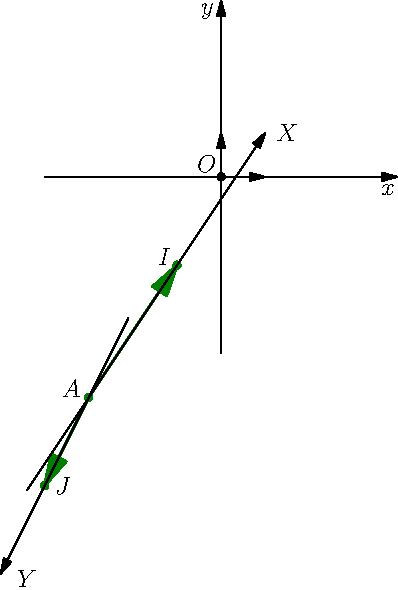
\includegraphics{C9895_1.pdf}
  % C9895_1.pdf: 198x198 px, 72dpi, 6.99x6.99 cm, bb=0 0 198 198
  \caption{Nouveau repère}
  \label{fig:C9895_1}
\end{figure}





% . Base affine. Coordonnées barycentriques. Sous-espace affine engendré par une partie. C'est l'intersection de tous les sous-espaces affines contenant cette partie. C'est aussi l'ensemble des barycentres des familles de points de la partie.

La notion d'\href{\baseurl C5727.pdf}{application affine} a bizarrement disparu du programme. 
\end{document}
